\begin{frame}
	\frametitle{Das Klimasystem - Zusammenfassung}

	\begin{figure}
		\centering
		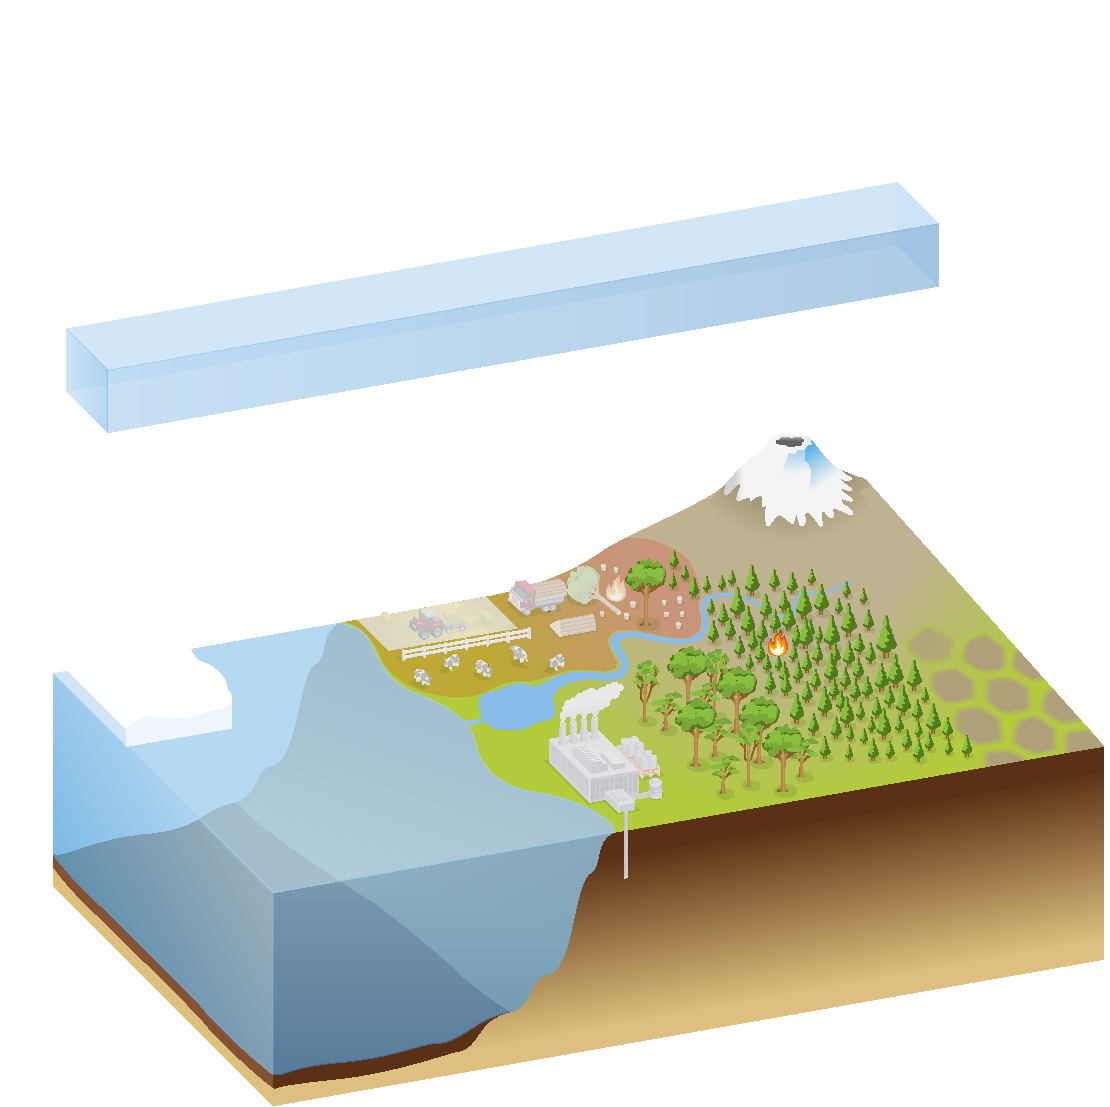
\includegraphics[trim={1cm 0cm 0cm 3cm}, clip, width=0.55\linewidth]{%
        bilder/climate_components/global_climate_components_spheres_ex_human.pdf}
		\caption{Abbildung des Klimasystems mit allen zuvor erklärten Elementen}
	\end{figure}

	\note{
		\begin{itemize}
			\item[] Abbildung mit allen zuvor erklärten Elementen
			\item[] das sind nur die größten Komponenten,
			\item[] viele kleinere Bereiche wie die Böden oder Elemente wie bestimmte Stoffkreisläufe sind ebenfalls wichtig
			\item[] es ist ein sehr komplexes System, an dem in vielen Stellen Änderungen und Wechselwirkungen auftreten
			\item[] also: komplexes System, mit komplexen Zusammenhängen
			\item[] in einzelnen Bereichen wie der Wolkenbildung sind noch Forschungsfragen offen
			\item[] (wir wollen Klarheit reinbringen, damit Lösungen eher im Kontext betrachtet werden können)
			\item[] (Eine Lösung kann nämlich Rückkopplungseffekte in anderen Bereichen erzeugen)
		\end{itemize}
	}
\end{frame}
